\section{Characterizing the Operational Safety Envelope}
\label{sec:eval}

This section empirically maps the operational safety envelope of edge-assisted control under delay and participant scaling. We express the envelope in terms of the freshness consumed by the planner at use time and normalize safety outcomes by distance traveled so that metrics remain comparable when the vehicle slows, stops early, or times out.

Our results proceed in four steps. (1) We characterize the delay process and the resulting AoI-at-use distribution at the planner boundary. (2) We measure the baseline envelope and show that the first collapse is a logic-induced consistency failure dominated by self-ghosting. (3) We show that increasing the number of participating egos shifts the system into the self-ghosting failure mode at lower delay because scaling inflates tails and increases duplication pressure. (4) We show that self-beacon anchoring expands the envelope by enforcing a publish-boundary ego-uniqueness contract, unmasking the physics-limited failure region.

\subsection{Methodology}
\subsubsection{Experimental Platform}
All experiments use \ecav~\cite{eCAV}, an open-source framework for edge-assisted CAV simulation built on CARLA~\cite{dosovitskiy_carla_nodate}. CARLA executes a full physics simulation (Unreal Engine 4 with NVIDIA PhysX) that captures vehicle mass, tire friction, braking forces, and steering limits. Tire-road interaction follows the Pacejka ``Magic Formula'' \cite{pacejka-book}. We run CARLA in synchronous mode with fixed step $\Delta t = 50$\,ms. All vehicles transmit at 20\,Hz and the edge publishes at the same quantum, so the control loop has a 50\,ms update cadence.

We execute experiments on a workstation (Intel i9-14900K, 192\,GB RAM, NVIDIA RTX 4080 Super). Synchronous simulation ensures deterministic replay under identical random seeds and latency traces.

\subsubsection{Scenarios}
We evaluate two occlusion-heavy scenarios derived from the NHTSA Pre-Crash Typology (PCT)~\cite{NHTSA_Typology}:

\begin{enumerate}[label=\arabic*.,noitemsep,topsep=0pt,leftmargin=1.2\parindent]
    \item \textbf{C-Left-Turn-Across-Path/Opposite-Direction (LTAP/OD):}
    an ego vehicle attempts an unprotected left turn at an unsignalized intersection with an occluded view of oncoming traffic (Fig.~\ref{fig:scenario_left_turn}).
    \item \textbf{B-Straight-Crossing-Path (SCP):}
    an ego vehicle attempts to overtake a stopped large vehicle while an oncoming vehicle is occluded (Fig.~\ref{fig:scenario_overtake}).
\end{enumerate}

\begin{figure}[h]
    \centering
    % Placeholder for the scenario diagram.
    \includegraphics[trim={5cm 5cm 0cm 0cm}, 
        clip,width=\columnwidth]{figures/occluded_left_turn.png}
    \caption{The Occluded Left-Turn Scenario involving two moving vehicles. The ego vehicle (blue) takes a blind left turn, intersecting with the white vehicle's trajectory. The overlaid blue tracks show the chronological progression of the single ego vehicle as it executes the turn. LTAP/OD Pre Crash Typology Code. %\KR{@Tyler: add more text to the caption so that it is clear that what is shown is the track of the ego vehicle in blue doing the left turn.  One could easily mistake there are 5 distinct cars in the picture shown.}
    }
    \label{fig:scenario_left_turn}
\end{figure}


\begin{figure}[h]
    \centering
    % Placeholder for the scenario diagram.
    \includegraphics[width=\columnwidth]{figures/blind_overtake_2.png}
    \caption{The Blind Overtake Scenario. The ego vehicle initiates an overtake of a large stopped vehicle while its view of oncoming traffic (white vehicle) is obstructed. SCP Overtake Pre Crash Typology Code.}
    \label{fig:scenario_overtake}
\end{figure}

\subsubsection{Single focal ego with participant scaling}
\label{sec:eval:scaling}

The safety objective is defined for a single \emph{focal} ego (the vehicle executing LTAP/OD or SCP). To address realism and edge contention, we add $N{-}1$ additional participating ego vehicles that also transmit beacons and perception outputs to the same edge server and receive per-ego publications. These additional egos increase state volume, association ambiguity, and shared edge/network contention without changing the focal task definition. We sweep $N \in \{1,2,4,8,16\}$ unless otherwise stated.

\subsubsection{Latency and AoI-at-use models}
\label{sec:e2e_lat_model}
We use two delay models. Both ultimately map to an observed AoI-at-use distribution at the planner boundary.

\paragraph{(1) Deterministic sweep (quantized delay).}
We apply a fixed end-to-end delay $L = k\cdot \Delta t$ with $k \in \mathbb{Z}_{\ge 0}$. This sweep isolates consistency failure modes by removing randomness in ordering.

\paragraph{(2) Trace-driven component delay.}
We use a per-tick component model:
\[
L \;=\; L_{\mathrm{veh}\rightarrow\mathrm{RSU}} \;+\; L_{\mathrm{backhaul}} \;+\; L_{\mathrm{proc}},
\]
where $L_{\mathrm{veh}\rightarrow\mathrm{RSU}}$ is sampled from SEE-V2X veh$\rightarrow$RSU RTT traces (resampled to $\Delta t$), $L_{\mathrm{backhaul}}$ is sampled from a log-normal fit whose median and $p_{99}$ match 5G-MOBIX field trials, and $L_{\mathrm{proc}}$ sums fixed stage latencies measured on our hardware. The reconciliation window $W$ in \S\ref{sec:timebase} is sized to cover high-percentile jitter under this model. We use this model for the packet-loss robustness study (Table~\ref{tab:loss_sensitivity}) and for the AoI-at-use characterization, where jitter-induced spread is visible in the CDF (Fig.~\ref{fig:aoi_cdf}).

\subsubsection{Baselines and VIPS Fidelity}
\label{sec:eval:baselines}
We compare three architectures: (1)~\textbf{Late Fusion}, a standard multi-camera pipeline that fuses independent detections without specific latency compensation; (2)~\textbf{Oracle}, an idealized single-source baseline that perfectly tracks all vehicles without cross-sensor duplication, isolating identity ambiguity from staleness; and (3)~\textbf{VIPS}~\cite{vips2022}, a latency-compensating architecture. Our VIPS implementation faithfully reproduces the core velocity-based temporal alignment (extrapolation) mechanism proposed in the literature to compensate for communication delay. While the original VIPS system also incorporates graph matching to align co-visible features, our focus is strictly on latency-induced state consistency. By isolating the temporal alignment mechanism, we demonstrate empirically that linear extrapolation fundamentally breaks down during dynamic maneuvers (e.g., sharp turns or acceleration), causing spatial mismatches that the edge cannot reconcile without a cryptographic identity invariant.

\subsubsection{Metrics: AoI-at-use, exposure normalization, and $S_{op}$}
\label{sec:eval:metrics}
\textbf{AoI-at-use at the planner boundary.}
Each edge-published object carries a generation timestamp. At the focal ego, we measure AoI-at-use
$\Delta_{\text{use}} = t_{\text{use}} - t_{\text{gen}}$ at the instant the planner consumes the object list. We report tail percentiles $p95(\Delta_{\text{use}})$ and $p99(\Delta_{\text{use}})$ per run. Reported ``latency'' values remain useful as configuration knobs, but the envelope is charted against observed $\Delta_{\text{use}}$ tails because tails capture reordering, queueing, and burst jitter.

\textbf{Exposure-normalized safety outcomes.}
Braking and slowdown metrics are reported as episodes and seconds per kilometer traveled by the focal ego, rather than per-tick counts. Per-km normalization prevents confounds when the focal ego slows, stops early, or times out. Each brake episode is labeled using simulator ground truth into one of three categories: (i) self-ghost, caused by a duplicate or misassociated focal-ego track; (ii) other false positive, caused by a non-focal spurious obstacle; or (iii) true positive, braking for a real hazard.

\textbf{Operational success.}
We define an operational success predicate for the focal run:
\[
S_{op} \;=\; S_{\text{coll}} \wedge S_{\text{ghost}} \wedge S_{\text{fp}} \wedge S_{\text{prog}},
\]
where $S_{\text{coll}}$ requires zero collisions, $S_{\text{ghost}}$ requires zero GT-labeled self-ghost brake episodes, $S_{\text{fp}}$ requires zero other false-positive brake episodes, and $S_{\text{prog}}$ requires average speed at least 60\% of the target speed (preventing survivors-by-freezing). We report $P(S_{op})$ and decompose component success probabilities to identify which constraint fails first.

\subsection{Results and Analysis}

\begin{figure*}[t]
\centering
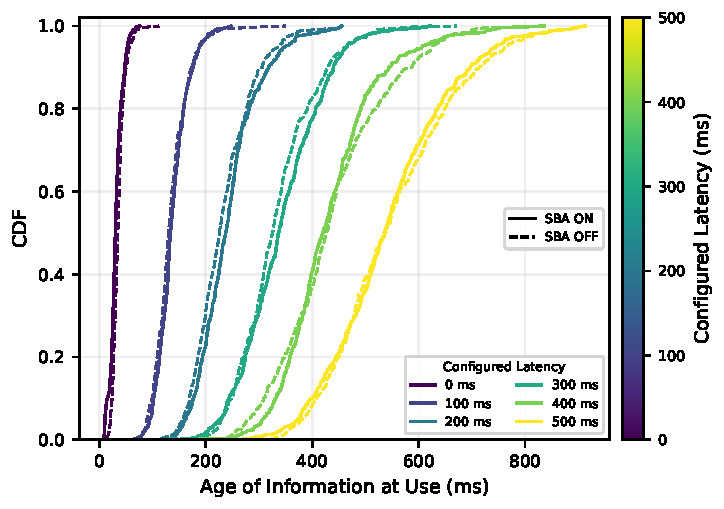
\includegraphics[width=\textwidth]{figures/aoi_cdf.pdf}
\caption{CDF of per-run $p99(\Delta_{\text{use}})$ across all configurations. The envelope index exhibits meaningful spread even at a fixed configured latency. SBA-on and SBA-off CDFs overlap for each manager, confirming that anchoring is an identity invariant, not a latency reduction.}
\label{fig:aoi_cdf}
\end{figure*}


\subsubsection{AoI-at-Use Characterization}
\label{sec:eval:aoi}

Figure~\ref{fig:aoi_cdf} shows the CDF of per-run $p99(\Delta_{\text{use}})$ across all configurations. Two observations are relevant. First, the envelope index $p99(\Delta_{\text{use}})$ exhibits meaningful spread even at a fixed configured latency, confirming that treating latency as a scalar is insufficient for envelope characterization. Second, SBA does not materially shift the AoI distribution. The SBA-on and SBA-off CDFs for each manager overlap, confirming that anchoring is an identity invariant rather than a latency reduction technique. Appendix Figure~\ref{fig:aoi_freshness} further shows that planner-side staleness ($\Delta_{\text{use}}^{\text{meas}}$) scales linearly with configured latency and dominates the total AoI, while model freshness ($\Delta_{\text{gen}}$) is bounded by the edge update loop. Together, these results justify indexing the envelope by $p99(\Delta_{\text{use}})$ rather than by nominal configured delay.

% float-aoi-freshness moved to Appendix~\ref{sec:appendix}

\begin{figure*}[t]
    \centering
    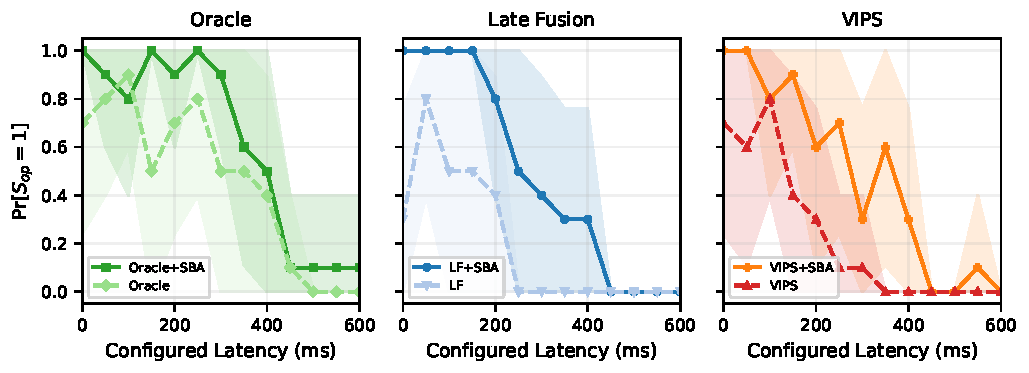
\includegraphics[width=\textwidth]{figures/success_vs_latency.pdf}
    \caption{Operational success $P(S_{op})$ vs.\ configured latency for each manager, with SBA on and off on the same axes. Late Fusion and VIPS exhibit a sharp safety cliff around ${\sim}100\text{--}150\,\mathrm{ms}$. Oracle maintains high $S_{op}$ until the physics-limited boundary at ${\sim}300\text{--}400\,\mathrm{ms}$. With SBA, the multi-source stacks track the Oracle curve.}
    \label{fig:success_vs_latency}
\end{figure*}


\subsubsection{Safety Envelope}
\label{sec:eval:envelope}

Figure~\ref{fig:success_vs_latency} plots $P(S_{op})$ against configured latency for each manager, with SBA on and off on the same axes. Late Fusion and VIPS both exhibit a sharp safety cliff: $P(S_{op})$ drops from near 1.0 to near 0 over a narrow latency range around ${\sim}100\text{--}150\,\mathrm{ms}$. The single-source Oracle does not exhibit self-ghosting and maintains high $S_{op}$ until the physics-limited boundary at ${\sim}300\text{--}400\,\mathrm{ms}$, where stale control inputs cause missed braking windows regardless of identity consistency. With SBA enabled, the multi-source stacks track the Oracle curve, shifting the cliff from the logic-limited boundary toward the physics-limited boundary.

\begin{figure*}[t]
\centering
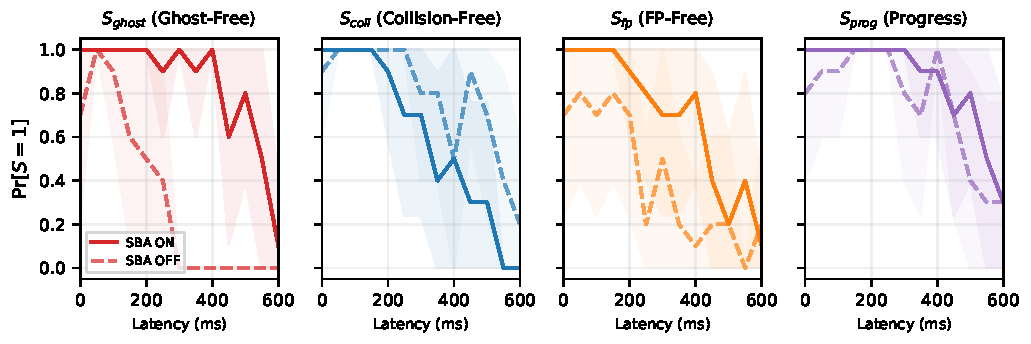
\includegraphics[width=\textwidth]{figures/failure_decomposition.pdf}
\caption{Component failure decomposition (Late Fusion) with SBA on (solid) and SBA off (dashed) overlaid on the same axes. Without SBA, $S_{\text{ghost}}$ is the first component to drop, confirming self-ghosting as the dominant early failure mode. With SBA, $S_{\text{ghost}}$ remains near 1.0 across all latencies and the binding constraint shifts to $S_{\text{coll}}$ or $S_{\text{prog}}$ at higher delay.}
\label{fig:failure_decomposition}
\end{figure*}

\begin{figure}[t]
\centering
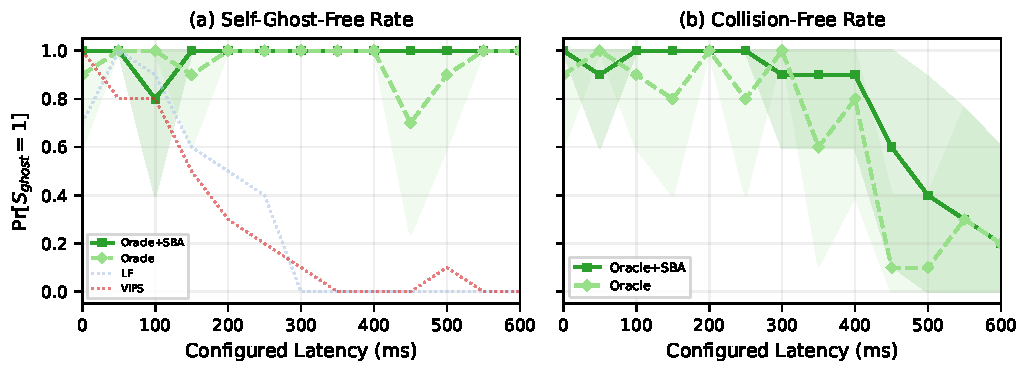
\includegraphics[width=\columnwidth]{figures/oracle_isolation.pdf}
\caption{Oracle baseline. (a) Self-ghost-free rate stays near 1.0 across all latencies, confirming that single-source perception eliminates ego-consistent duplicates by construction. (b) Collision-free rate degrades at high latency due to physics. The gap between the Oracle physics bound and the multi-source logic cliff quantifies the cost of identity ambiguity.}
\label{fig:oracle_isolation}
\end{figure}


\subsubsection{Failure Decomposition and Oracle Isolation}
\label{sec:eval:decomposition}

Figure~\ref{fig:failure_decomposition} decomposes $P(S_{op})$ into its four components ($S_{\text{coll}}$, $S_{\text{ghost}}$, $S_{\text{fp}}$, $S_{\text{prog}}$) as a function of latency. For the multi-source stacks without SBA, $S_{\text{ghost}}$ is the first component to drop, confirming that self-ghosting is the dominant early failure mode. With SBA enabled, $S_{\text{ghost}}$ remains at or near 1.0 across all tested latencies, and the binding constraint shifts to $S_{\text{coll}}$ or $S_{\text{prog}}$ at higher delay.

The Oracle baseline provides direct evidence that the early cliff is structural, not an artifact of tracker tuning or heuristic thresholds. Oracle uses the same AB3DMOT tracker, the same Kalman filter, and the same prediction pipeline as the multi-source stacks. The only difference is its input: one detection per physical actor per tick, with no cross-camera or cross-sensor duplicates. Because it never generates ego-consistent duplicates, it satisfies condition~(i) of Section~\ref{sec:beacon} by construction. Figure~\ref{fig:oracle_isolation} confirms that Oracle maintains $P(S_{\text{ghost}} = 1) \approx 1.0$ across all latencies, while its collision-free rate degrades at high latency due to physics. The gap between where Oracle fails at the physics bound and where the multi-source stacks fail at the logic cliff quantifies the cost of multi-source identity ambiguity. This isolation confirms that the early cliff arises from multi-source disagreement, not from staleness alone.

\begin{figure*}[t]
\centering
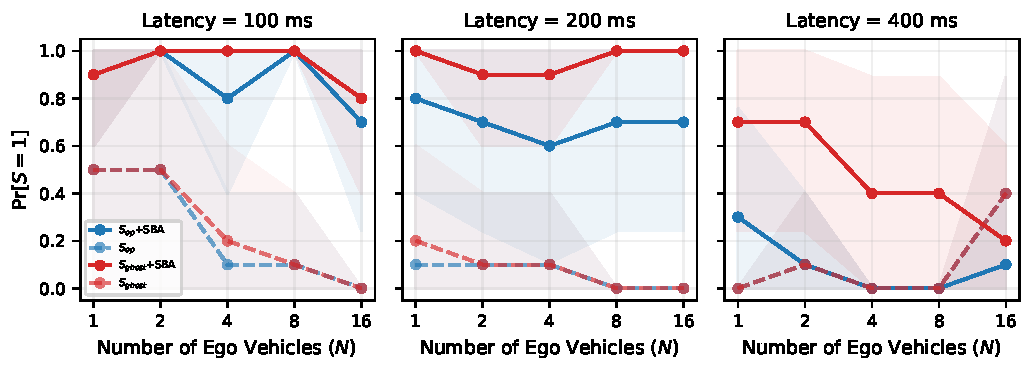
\includegraphics[width=\textwidth]{figures/multi_ego_scaling.pdf}
\caption{Multi-ego scaling (Late Fusion) at representative latencies. $S_{op}$ (blue) and $S_{\text{ghost}}$ (red) vs.\ ego count $N$, with SBA on (solid) and SBA off (dashed) overlaid. Without SBA, self-ghost brakes rise sharply for $N \geq 4$ and operational success collapses. With SBA, both metrics remain high across all tested $N$, tracking the physics-limited baseline.}
\label{fig:multi_ego_scaling}
\end{figure*}


\subsubsection{Multi-Ego Scaling}
\label{sec:eval:scaling_results}

Figure~\ref{fig:multi_ego_scaling} shows $P(S_{op})$ and $P(S_{\text{ghost}})$ as a function of ego count $N$ at representative latencies, with SBA on and off overlaid on the same axes. Without SBA, self-ghost brakes are near zero at $N \in \{1, 2\}$ and rise sharply for $N \geq 4$. With SBA, the self-ghost-free rate remains high across all tested $N$, and operational success degrades more gradually.

\begin{figure}[t]
\centering
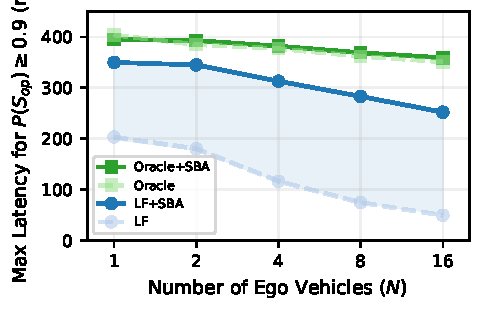
\includegraphics[width=\columnwidth]{figures/envelope_boundary.pdf}
\caption{Safety envelope boundary: maximum end-to-end latency at which $P(S_{op}) \geq 0.9$, as a function of the number of participating ego vehicles $N$. Solid lines show SBA on, dashed lines show SBA off. The shaded region for Late Fusion shows the envelope expansion from anchoring. Without SBA, the tolerable latency for multi-source stacks collapses from ${\sim}200\,\mathrm{ms}$ at $N{=}1$ to ${\sim}50\,\mathrm{ms}$ at $N{=}16$. With SBA, it degrades gradually from ${\sim}350\,\mathrm{ms}$ to ${\sim}250\,\mathrm{ms}$.}
\label{fig:envelope_boundary}
\end{figure}


Figure~\ref{fig:envelope_boundary} summarizes this as a single envelope boundary curve: the maximum latency at which $P(S_{op}) \geq 0.9$, plotted against $N$. Without SBA, the tolerable latency for multi-source stacks collapses from ${\sim}200\,\mathrm{ms}$ at $N{=}1$ to ${\sim}50\,\mathrm{ms}$ at $N{=}16$. With SBA, the boundary degrades gradually from ${\sim}350\,\mathrm{ms}$ to ${\sim}250\,\mathrm{ms}$, tracking the Oracle curve. The shaded gap quantifies the envelope expansion that anchoring provides across participant counts.

Appendix Figure~\ref{fig:duplicate_clusters} shows the root cause: pre-NMS duplicate clusters per tick grow with $N$ for the camera-driven managers, while Oracle stays at zero. More participating vehicles produce more overlapping fields of view, generating more near-duplicate hypotheses that the tracker must disambiguate. Under asynchronous delivery, duplicates that survive NMS can birth ego-like tracks, creating self-ghosting opportunities that scale with $N$. The first-failure categorization in Appendix Figure~\ref{fig:first_failure} confirms that as $N$ increases, self-ghosting becomes the dominant failure mode for multi-source stacks without SBA, while Oracle transitions to physics-limited failures regardless of $N$.

% float-duplicate-clusters and float-first-failure moved to Appendix~\ref{sec:appendix}

\subsubsection{Anchoring Efficacy}
\label{sec:eval:anchoring}

Figure~\ref{fig:brake_provenance} decomposes the focal ego's brake ticks by GT-labeled provenance (self-ghost, NPC hazard, parked car, unknown). Without SBA, the self-ghost fraction grows with latency and $N$. With SBA, self-ghost brakes are eliminated and the remaining braking is dominated by true-positive responses to real hazards. Appendix Figure~\ref{fig:brake_episodes_km} normalizes by distance traveled and confirms that the self-ghost and other-FP brake rates remain low at low latency and increase primarily in configurations where identity consistency is stressed. Appendix Figure~\ref{fig:ego_uniqueness} shows ego-uniqueness violations (ticks where the tracker maintains more than one ego-consistent track) as a function of $N$: violations grow with $N$ for both Late Fusion and VIPS without SBA, and SBA suppresses them.

\begin{figure}[t]
\centering
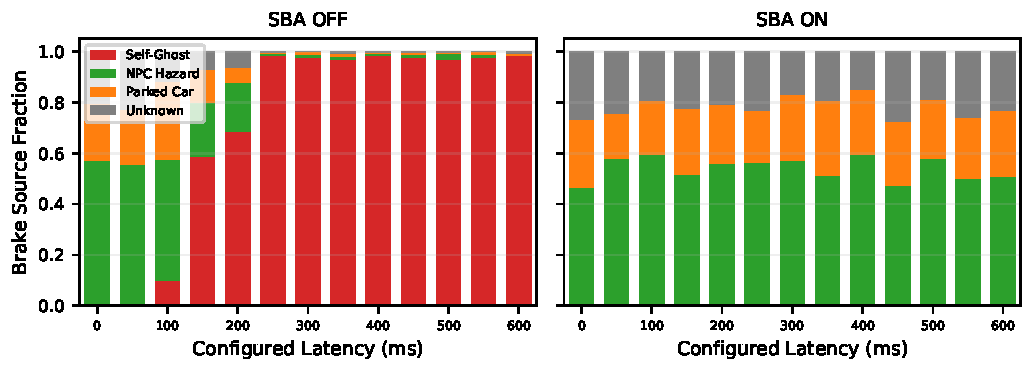
\includegraphics[width=\columnwidth]{figures/brake_provenance.pdf}
\caption{Brake provenance breakdown (Late Fusion) by GT-labeled category: self-ghost, NPC hazard, parked car, and unknown. Without SBA (left), the self-ghost fraction grows with latency. With SBA (right), self-ghost brakes are eliminated and remaining braking is dominated by true-positive responses.}
\label{fig:brake_provenance}
\end{figure}

% float-brake-episodes-km and float-ego-uniqueness moved to Appendix~\ref{sec:appendix}

\subsubsection{System Overhead}
\label{sec:eval:overhead}

Table~\ref{tab:bandwidth} summarizes per-vehicle bandwidth. Each vehicle transmits a 96\,B self-beacon and a variable-length list of 3-D bounding boxes at 20\,Hz. Across all evaluation frames, no vehicle transmitted more than ten boxes, and the empirical mean was seven. The worst-case uplink is ${\approx}9.9\;\mathrm{KB/s}$ per vehicle, one to two orders of magnitude below intermediate-feature systems such as V2X-ViT (${\sim}1.3\;\mathrm{MB/s}$~\cite{v2xvit2022}) and three orders below raw-LiDAR systems such as EMP (${\sim}3.7\;\mathrm{MB/s}$~\cite{EMP}).

Appendix Figure~\ref{fig:latency_breakdown_combined} shows per-component processing latency. Vehicle-side perception (YOLOv5) dominates at ${\sim}25\,\mathrm{ms}$ median. Edge-side processing is an order of magnitude faster in sparse scenes. The overhead of the anchoring logic is negligible: a median increase of 0.2\,ms over the baseline tracker. Appendix Figure~\ref{fig:scalability} shows tracker latency as a function of the number of concurrent objects, reaching 35\,ms at 200 objects.

\begin{table}[t]
\footnotesize
\centering
\caption{Per-vehicle uplink budget at \textbf{20 Hz}.
         Statistics computed over all frames in both scenarios
         (\(n\!=\!2{,}000\)); each vehicle sent at most 10 boxes per frame.}
\label{tab:bandwidth}
\begin{tabularx}{\linewidth}{@{}lccc@{}}
\toprule
\textbf{Msg type} & \textbf{Avg.\ size (B)} & \textbf{p95 (B)} & \textbf{KB/s}\\
\midrule
Self-beacon (fixed)        & 96   & 96    & 1.88 \\
3-D bbox list ($\leq$10 boxes)  & 4,130 & 4,720 & 8.06 \\
\midrule
\textbf{Total}             & —    & —     & \textbf{9.94} \\
\bottomrule
\end{tabularx}
%\vspace{-0.6em}
\end{table}
% float-latency-breakdowns and float-scalability moved to Appendix~\ref{sec:appendix}

\subsubsection{Packet Loss Robustness}
\label{sec:eval:loss}

Table~\ref{tab:loss_sensitivity} reports anchoring success rate under the hybrid 190\,ms latency model as a function of PC5 link loss. Anchoring maintains 100\% success at up to 10\% loss and degrades at 12\% and above. The SEE-V2X dataset reports $\leq 5\%$ loss for real RSU links~\cite{seev2x}, indicating at least a $2\times$ reliability margin under field conditions.

\begin{table}[t]
\footnotesize
\centering
\caption{Anchoring success rate under the hybrid 190\,ms latency model (20 runs).}
\label{tab:loss_sensitivity}
\begin{tabularx}{\linewidth}{@{}l*{5}{>{\centering\arraybackslash}X}@{}}
\toprule
\textbf{PC5 loss (\%)} & 0 & 5 & 10 & 12 & 15 \\ \midrule
Success rate (\%)      & 100 & 100 & 100 & 80 & 5 \\ \bottomrule
\end{tabularx}
\end{table}


\subsubsection{GNSS Noise Robustness}
\label{sec:eval:gnss}

Without SBA, the ego vehicle identifies its own track by spatial proximity: it matches its GNSS position to the nearest tracker output within a gating radius. This spatial self-identification is sensitive to GNSS position noise. As noise increases, the match becomes unreliable and the ego can fail to recognize its own track, triggering self-ghosting even at low latency.

SBA decouples self-identification from position accuracy. The beacon carries an authoritative vehicle ID that the edge binds to the ego track regardless of spatial distance. The ego's identity is established by the ID match, not by the position match.

Figure~\ref{fig:gnss_robustness} shows $P(S_{op})$ as a function of GNSS position noise (standard deviation $\sigma$) at 200\,ms configured latency. Without SBA, multi-source stacks degrade rapidly once $\sigma$ exceeds ${\sim}2\,\mathrm{m}$. With SBA, operational success remains high until $\sigma$ exceeds ${\sim}5\,\mathrm{m}$, well beyond the ${\sim}1\text{--}3\,\mathrm{m}$ accuracy of consumer-grade GNSS receivers in urban environments. Oracle is less affected in the SBA-off condition because it has no multi-source duplicates, but it still degrades at high noise levels because stale position estimates distort predicted trajectories.

\begin{figure}[t]
\centering
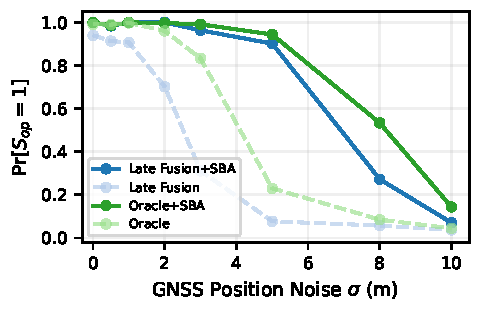
\includegraphics[width=\columnwidth]{figures/gnss_noise_robustness.pdf}
\caption{Operational success vs.\ GNSS position noise (standard deviation $\sigma$ in metres), at 200\,ms configured latency with $N{=}1$. Without SBA (left), spatial-only self-identification degrades rapidly once $\sigma$ exceeds ${\sim}2\,\mathrm{m}$. With SBA (right), the beacon carries an authoritative identity that does not depend on position accuracy, and operational success remains high until $\sigma$ exceeds ${\sim}5\,\mathrm{m}$.}
\label{fig:gnss_robustness}
\end{figure}

